	\section*{Exercice 3 (5 points)}
	

	

	
	\subsection*{1. Exprimer par une phrase l’information donnée par le nombre 0,6 sur la branche de \(B_1\) à \(C\).}
	
	« La probabilité que le cookie soit au chocolat, sachant qu’il provient de la boulangerie 1 est égale à $0,6$. »
	
	\subsection*{2. Recopier et compléter sur la copie l’arbre pondéré ci-dessus.}
	
	\begin{center}
	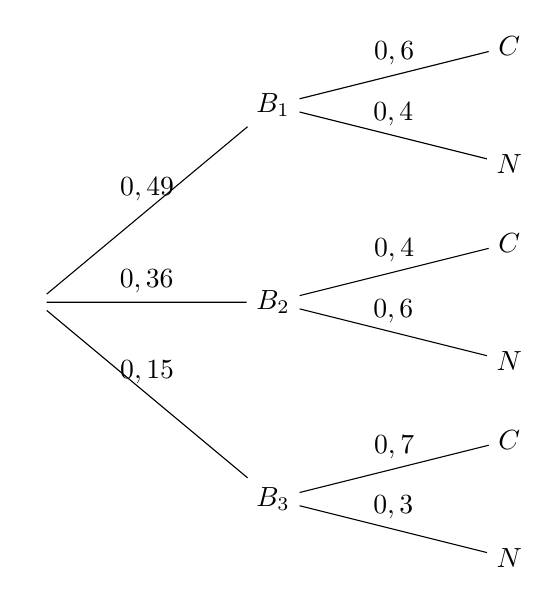
\begin{tikzpicture}
		[level 1/.style={level distance=3cm,
			sibling distance=2.5cm},
		level 2/.style={level distance=3cm,
			sibling distance=1.5cm}
	]
		\node {} [grow'=right]
		child {node {$B_1$}
			child {node {$C$}
				edge from parent node[above] {$0,6$}
			}
			child {node {$N$}
				edge from parent node[above] {$0,4$}
				}
			edge from parent node[above] {$0,49$}
		}
		child {node {$B_2$}
			child {node {$C$}
				edge from parent node[above] {$0,4$}
			}
			child {node {$N$}
				edge from parent node[above] {$0,6$}
			}
			edge from parent node[above] {$0,36$}
		}
		child {node {$B_3$}
			child {node {$C$}
				edge from parent node[above] {$0,7$}
			}
			child {node {$N$}
				edge from parent node[above] {$0,3$}
			}
			edge from parent node[above] {$0,15$}
		}
		;
	\end{tikzpicture}
\end{center}
	
	\subsection*{3. Définir par une phrase l’évènement \(B_1 \cap C\) et calculer sa probabilité.}
	
	\(B_1 \cap C\) est l’évènement : « le cookie vient de la boulangerie 1 et est au chocolat ».
	\[ P(B_1 \cap C) = P(B_1) \times P_{B_1}(C) = 0,49 \times 0,6 = 0,294. \]
	
	\subsection*{4. Montrer la probabilité \(P(C)\) d’avoir un cookie au chocolat est égale à 0,543.}
	
	D’après la loi des probabilités totales :
	\begin{align*}
		P(C) &= P(B_1 \cap C) + P(B_2 \cap C) + P(B_3 \cap C)\\
		& = P(B_1) \times P_{B_1}(C) + P(B_2) \times P_{B_2}(C) + P(B_3) \times P_{B_3}(C) \\
		& = 0,49 \times 0,6 + 0,36 \times 0,4 + 0,15 \times 0,7 \\
	& = 0,294 + 0,144 + 0,105 \\
	&= 0,543. 
	\end{align*}
	
	\subsection*{5. Calculer la probabilité d’avoir un cookie provenant de la boulangerie 2 sachant qu’il est au chocolat. On donnera le résultat arrondi au millième.}
	
	Il faut trouver \(P_C(B_2)\) :
	\[ P_C(B_2) = \dfrac{P(C \cap B_2)}{P(C)} = \dfrac{0,144}{0,543} \approx 0,2651, \]
	soit 0,265 au millième près.
	
